\section{Risultati}\label{sec:risultati}
  I risultati ottenuti sono riassunti nella tabella \ref{tab : risultati}. I valori numerici dei dati raccolti sono riportati in appendice \ref{sec:valori-misure}. Il grafico in figura \ref{fig : dati raccolti} rappresenta le osservazioni effettuate con sovraimpressi i \emph{fit}.
  \begin{table}[H]
    \centering
    \begin{tabular}{c | c  c  c }[t]
      & $-100 \: mA$ & $-150 \: mA$ & $-200 mA$ \\
      \hline
      Conduttività & $(17.81 \pm 0.06) \: \Omega^{-1}$ & $(24.34 \pm 0.08) \: \Omega^{-1}$ & $(30.62 \pm 0.11) \: \Omega^{-1}$ \\
      $\beta$ ($-3 \: V$) & $0.544 \pm 0.002$ & $0.4955 \pm 0.0019$ & $0.4689 \pm 0.0019$ \\
      Tensione di Early & $(0.0561 \pm 0.0019) \: V$ & $(0.0534 \pm 0.0018) \: V$ & $(0.0627 \pm 0.0019) \: V$ \\
      \hline
    \end{tabular}
    \caption{\emph{Valori di caratteristica misurati e rispettivi valori di corrente di base.}}
    \label{tab : risultati}
  \end{table}

  \begin{figure}
    \centering
    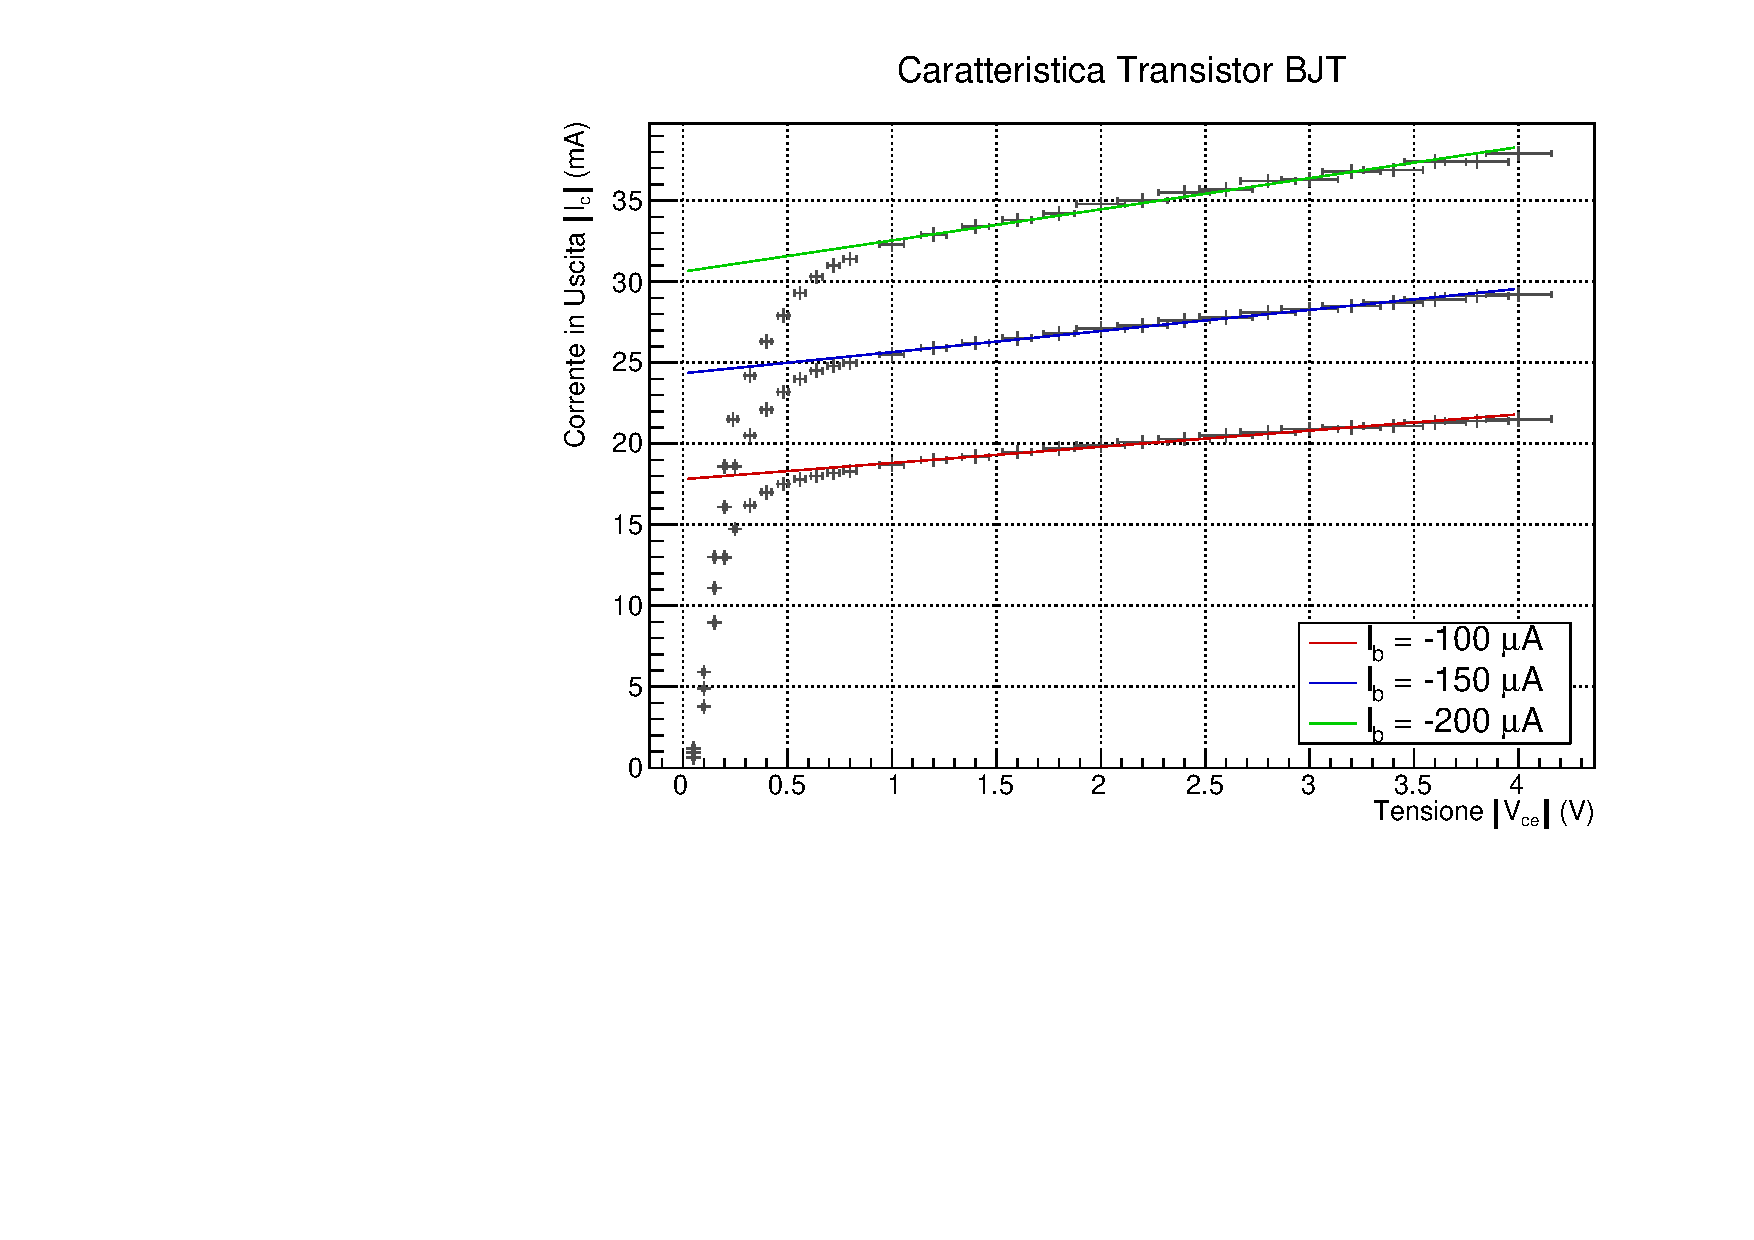
\includegraphics[width=\textwidth]{../assets/GraficoTot.pdf}
    \caption{\emph{Dati raccolti con relativo fit lineare. In tutti e tre i casi il fit è stato svolto per valori di tensione $\left|V_{ce}\right| >= 1$.}}
    \label{fig : dati raccolti}
  \end{figure}
